\documentclass{article}
\usepackage{graphicx,amsmath}

\begin{document}
\title{Today and before in a train of thought: exploring the time variation of the best choice finf}
\author{Steven Dorsher}
\maketitle


I have plotted Finf over time from 380 M to 690 M for several modes between 0 and 31. The higher modes (sampled at 10, 15, 20, and 30) seem to evolve smoothly. Lower modes seem to have discontinuities, though not every mode. In particular, mode 4 has two point discontinuities right before perihelion and aphelion. Mode 5 has two step disctoninuities right before perihelion and aphelion as well. Mode 7 has step discontinuities at the start and just after aphelion. Mode 27 has a small bump feature just after apastron. Mode 28 and 29 has a larger bump in the same place. Mode 30 has two point discontinuities before and after apastron (the bump has split). Mode 31 also has two bumps to either side of apastron, that are nearly point discontinuities. It also has a bump just before perihelion. {\em All mode numbering is off by one. It is the end of the day and I am not going to fix this. When I say ``Mode 30'' please mentally subtract one and read ``Mode 29''.}

These plots are made using the data in nmaxFinfOverTime\_finf.csv, generated by running sh finfnmaxscript2 380 610 10 (before I broke it by adding a fourth argument). This calls readtimeandprint.py which reads bestfinfoverinitorder???.csv for all times and generates a file containing either nmax or finf in transposed order, listed by time, for the purposes of plotting one mode at a time in gnuplot as a function of time. bestfinf... is generated using bestfinfscript, which calls bestfinfselector.py if the files don't already exist then calls fitcoefftable.py to produce a surface plot. 

It is likely the discontinuities I discovered today are what is causing the problems with the self force evolution I plotted yesterday. The self force evolution is also shown below, at the bottom. As you can see, it makes no difference whether three terms or four terms are included in the fit over l-modes to determine the self force summed to infinite l-mode. 

\section{Yesterday and before}

The self force evolution is generated from selfForceOverTimeSinglePoint4term.csv, selfForceOverTimeAvgSmallRange3Term.csv, and selfForceOverTimeAvgSmallRange4Term.csv. These were generated using bestfinfscript for various command line arguments. Averaging over a small range means using lmin between 14 and 17 and lmax between 22 and 25, then averaging the self force over the surface that results. Averaging over a large range means the same thing, but with lmin between 14 and 19 and lmax between 24 and 30. Selecting the self force at a single point means choosing the value at the center of the the rectangle formed by the surface chosen, with a bias toward lower values when evenly divisible by two. I should also consider choosing points at the widest values of the small range; however, in the large range, it is clear this would result in problems with roundoff noise, due to the steep changes in the slope of the surface. See plots below. 


\section{Next}

I need to recheck the order extrapolation plots, which I have now made hard to run. I need to re-enable them, which should not be too difficult (I think). Some previous versions are given below. extrapolate7.py used to be used to do this, but now is too automated. It may be possible to run it in a less automated mode. fitcoefftable.py can take output from extrapolate7.py or bestfinfselector.py, depending on whether you want to choose the best finf based on which mode is the last to produce a valid number (instead of a nan) or if you want to choose using a single order. If you use a single order across all modes, there needs to be some way to determine how to ignore the nans and still sum the modes. This is why I'm trying to plot the values of nmax for finfnmaxscript2's output, but I haven't succeeded yet because it won't run. Tomorrow. 


\section{Plots from today}

\begin{figure}
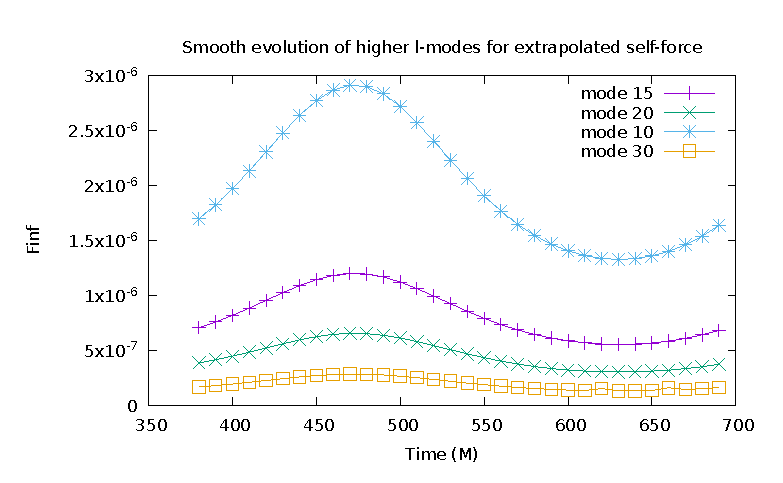
\includegraphics{finfOverTimeHighL}
\end{figure}
\begin{figure}
\includegraphics{finfOverTimeL4}
\end{figure}
\begin{figure}
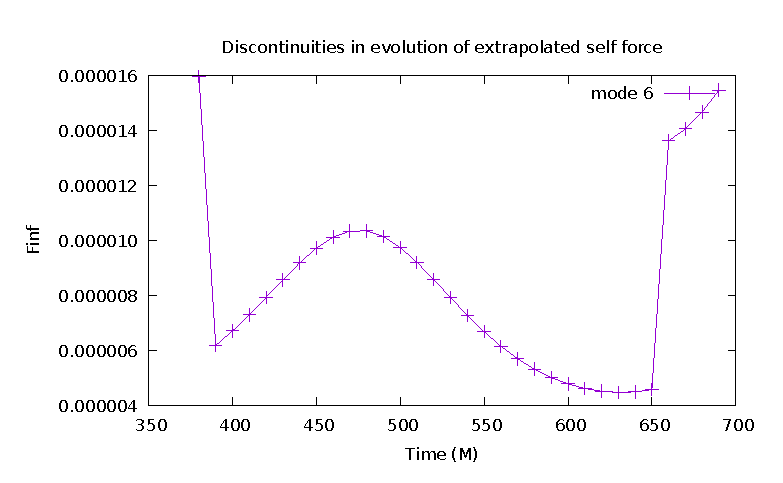
\includegraphics{finfOverTimeL6}
\end{figure}
\begin{figure}
\includegraphics{finfOverTimeL29}
\end{figure}
\begin{figure}
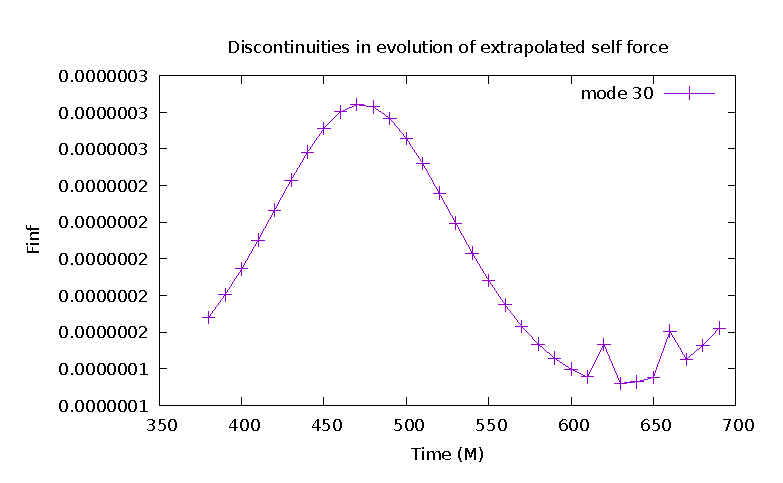
\includegraphics{finfOverTimeL30}
\end{figure}

\begin{figure}
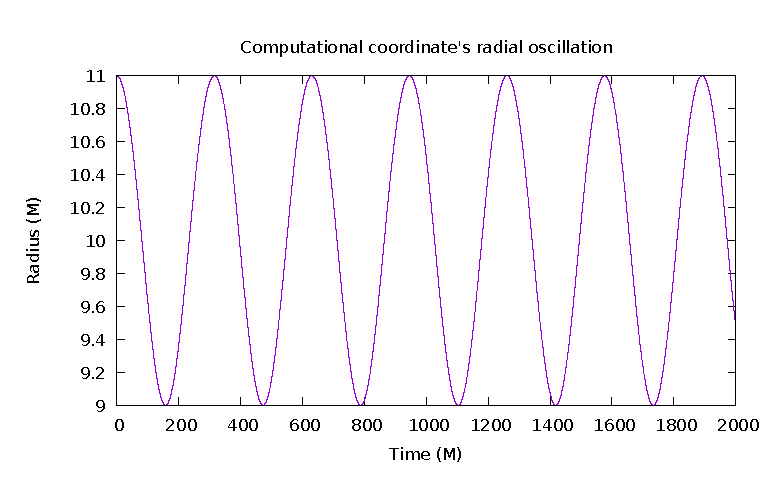
\includegraphics{orbit}
\end{figure}


\begin{figure}
  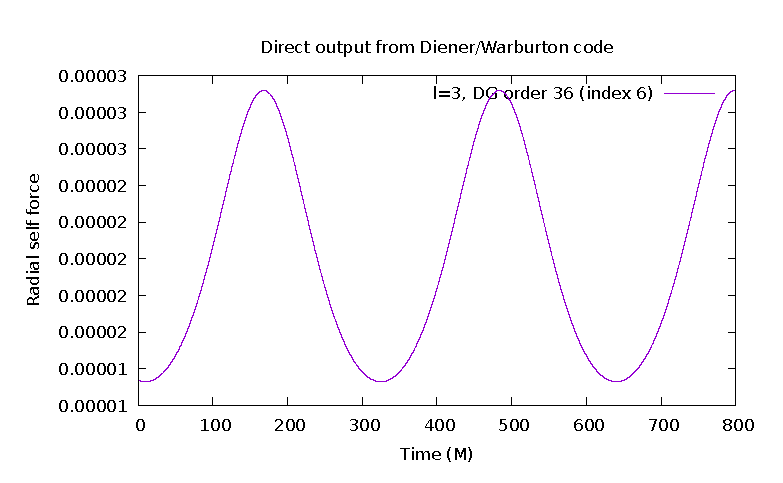
\includegraphics{psirl_l3_order36}
  \caption{470 M near perihelion, 640 M at aphelion}
\end{figure}

\section{Plots from yesterday and before}

\begin{figure}
  \includegraphics{selfforceavgsmallrange3term}
\end{figure}
\begin{figure}
  \includegraphics{selfforceavgsmallrange4term}
\end{figure}

\begin{figure}
  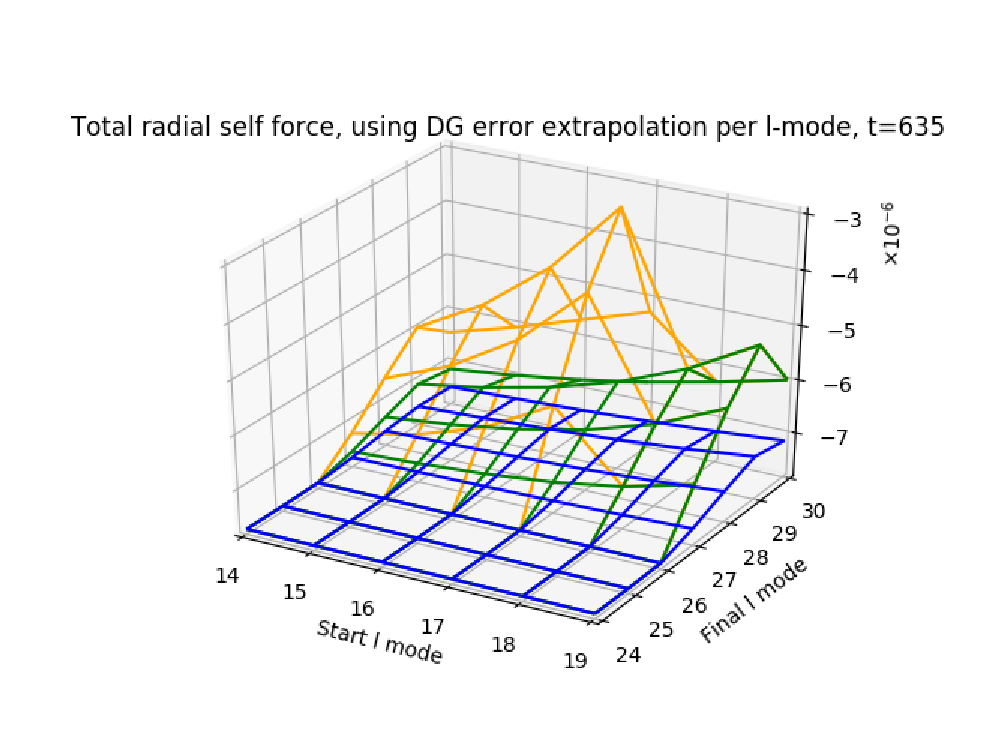
\includegraphics{bestfinflminlmax234terms635fullrange_perihelion}
\caption{Aphelion large range has roundoff noise at high lmax}
\end{figure}

\begin{figure}
  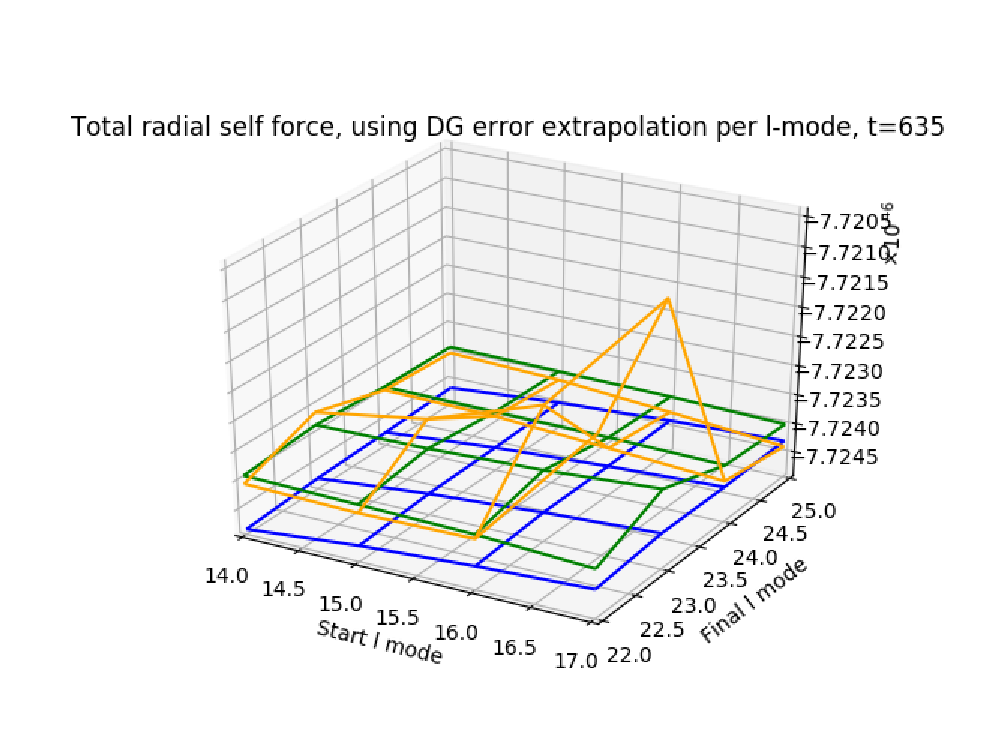
\includegraphics{bestfinflminlmax234termst635smallrange_perihelion}
\caption{Aphelion small range shows no roundoff noise}
\end{figure}


\begin{figure}
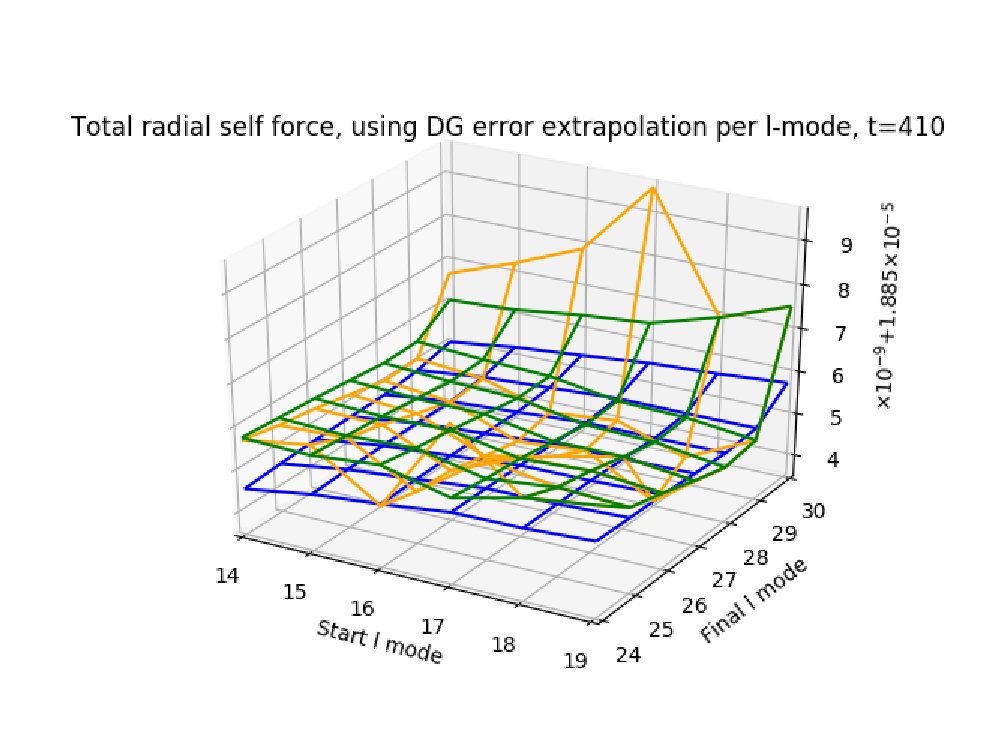
\includegraphics{bestfinflminlmax234termst410fullrange}
\caption{Small roundoff noise in full range at time 410 M}
\end{figure}

\begin{figure}
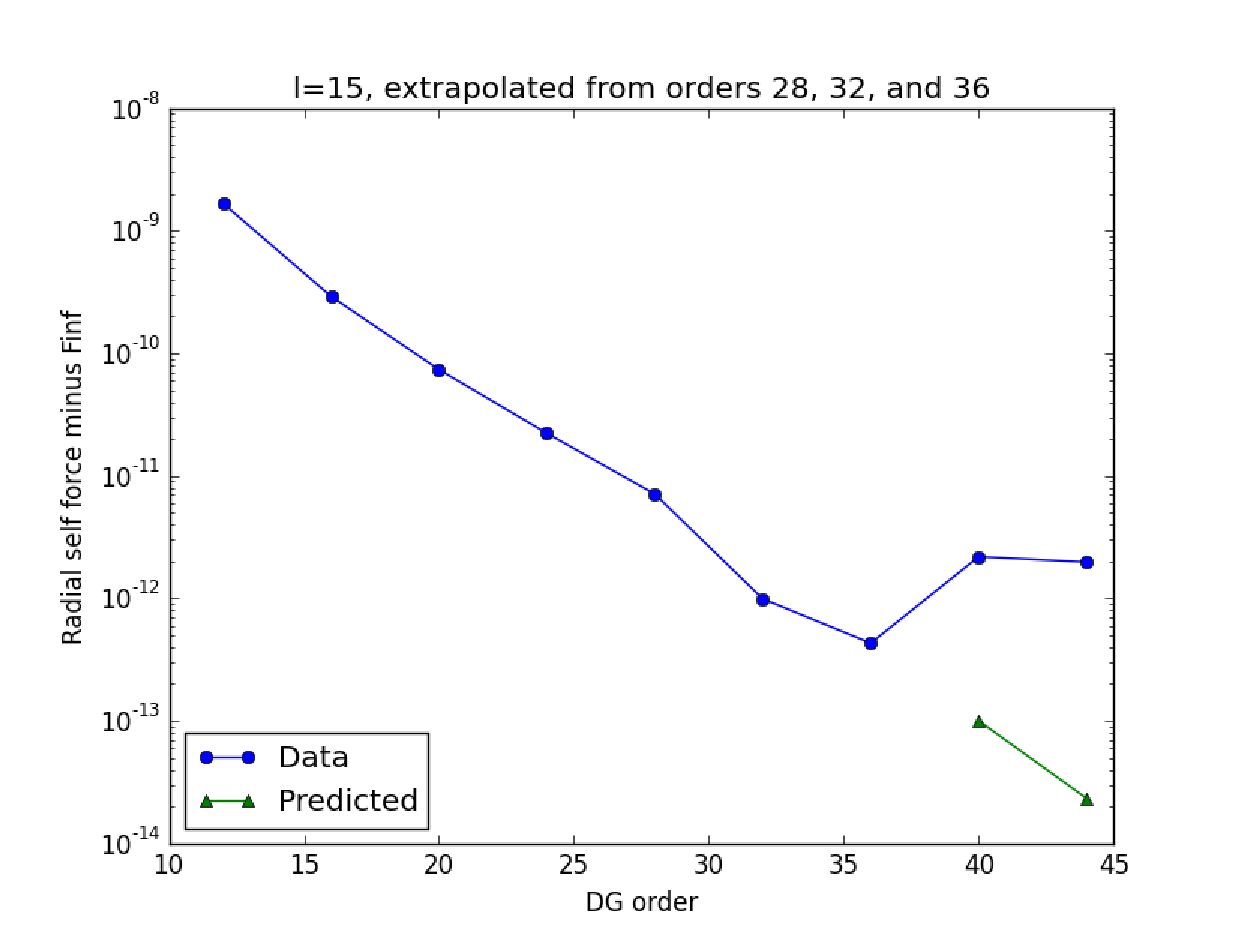
\includegraphics{extrapolate7plot}
\end{figure}


\end{document}
